%!TEX root = ../my_thesis.tex
\section{The Standard Model of particle physics}
\label{sec:sm}

The \emph{Standard Model} (SM) of particle physics \cite{Salam, Weinberg, Glashow} is a \emph{non-abelian, Yang-Mills quantum field theory} based on the $SU(3)\times SU(2)\times U(1)$ 
gauge symmetry group. This model provides a coherent, unified and experimentally-established picture of electromagnetic, weak and strong interactions, as well as
a description of the known elementary particles (quarks, leptons, gauge bosons and Higgs boson, Fig.~\ref{fig:particles}).

\begin{figure}[htbp]
  \begin{center}
    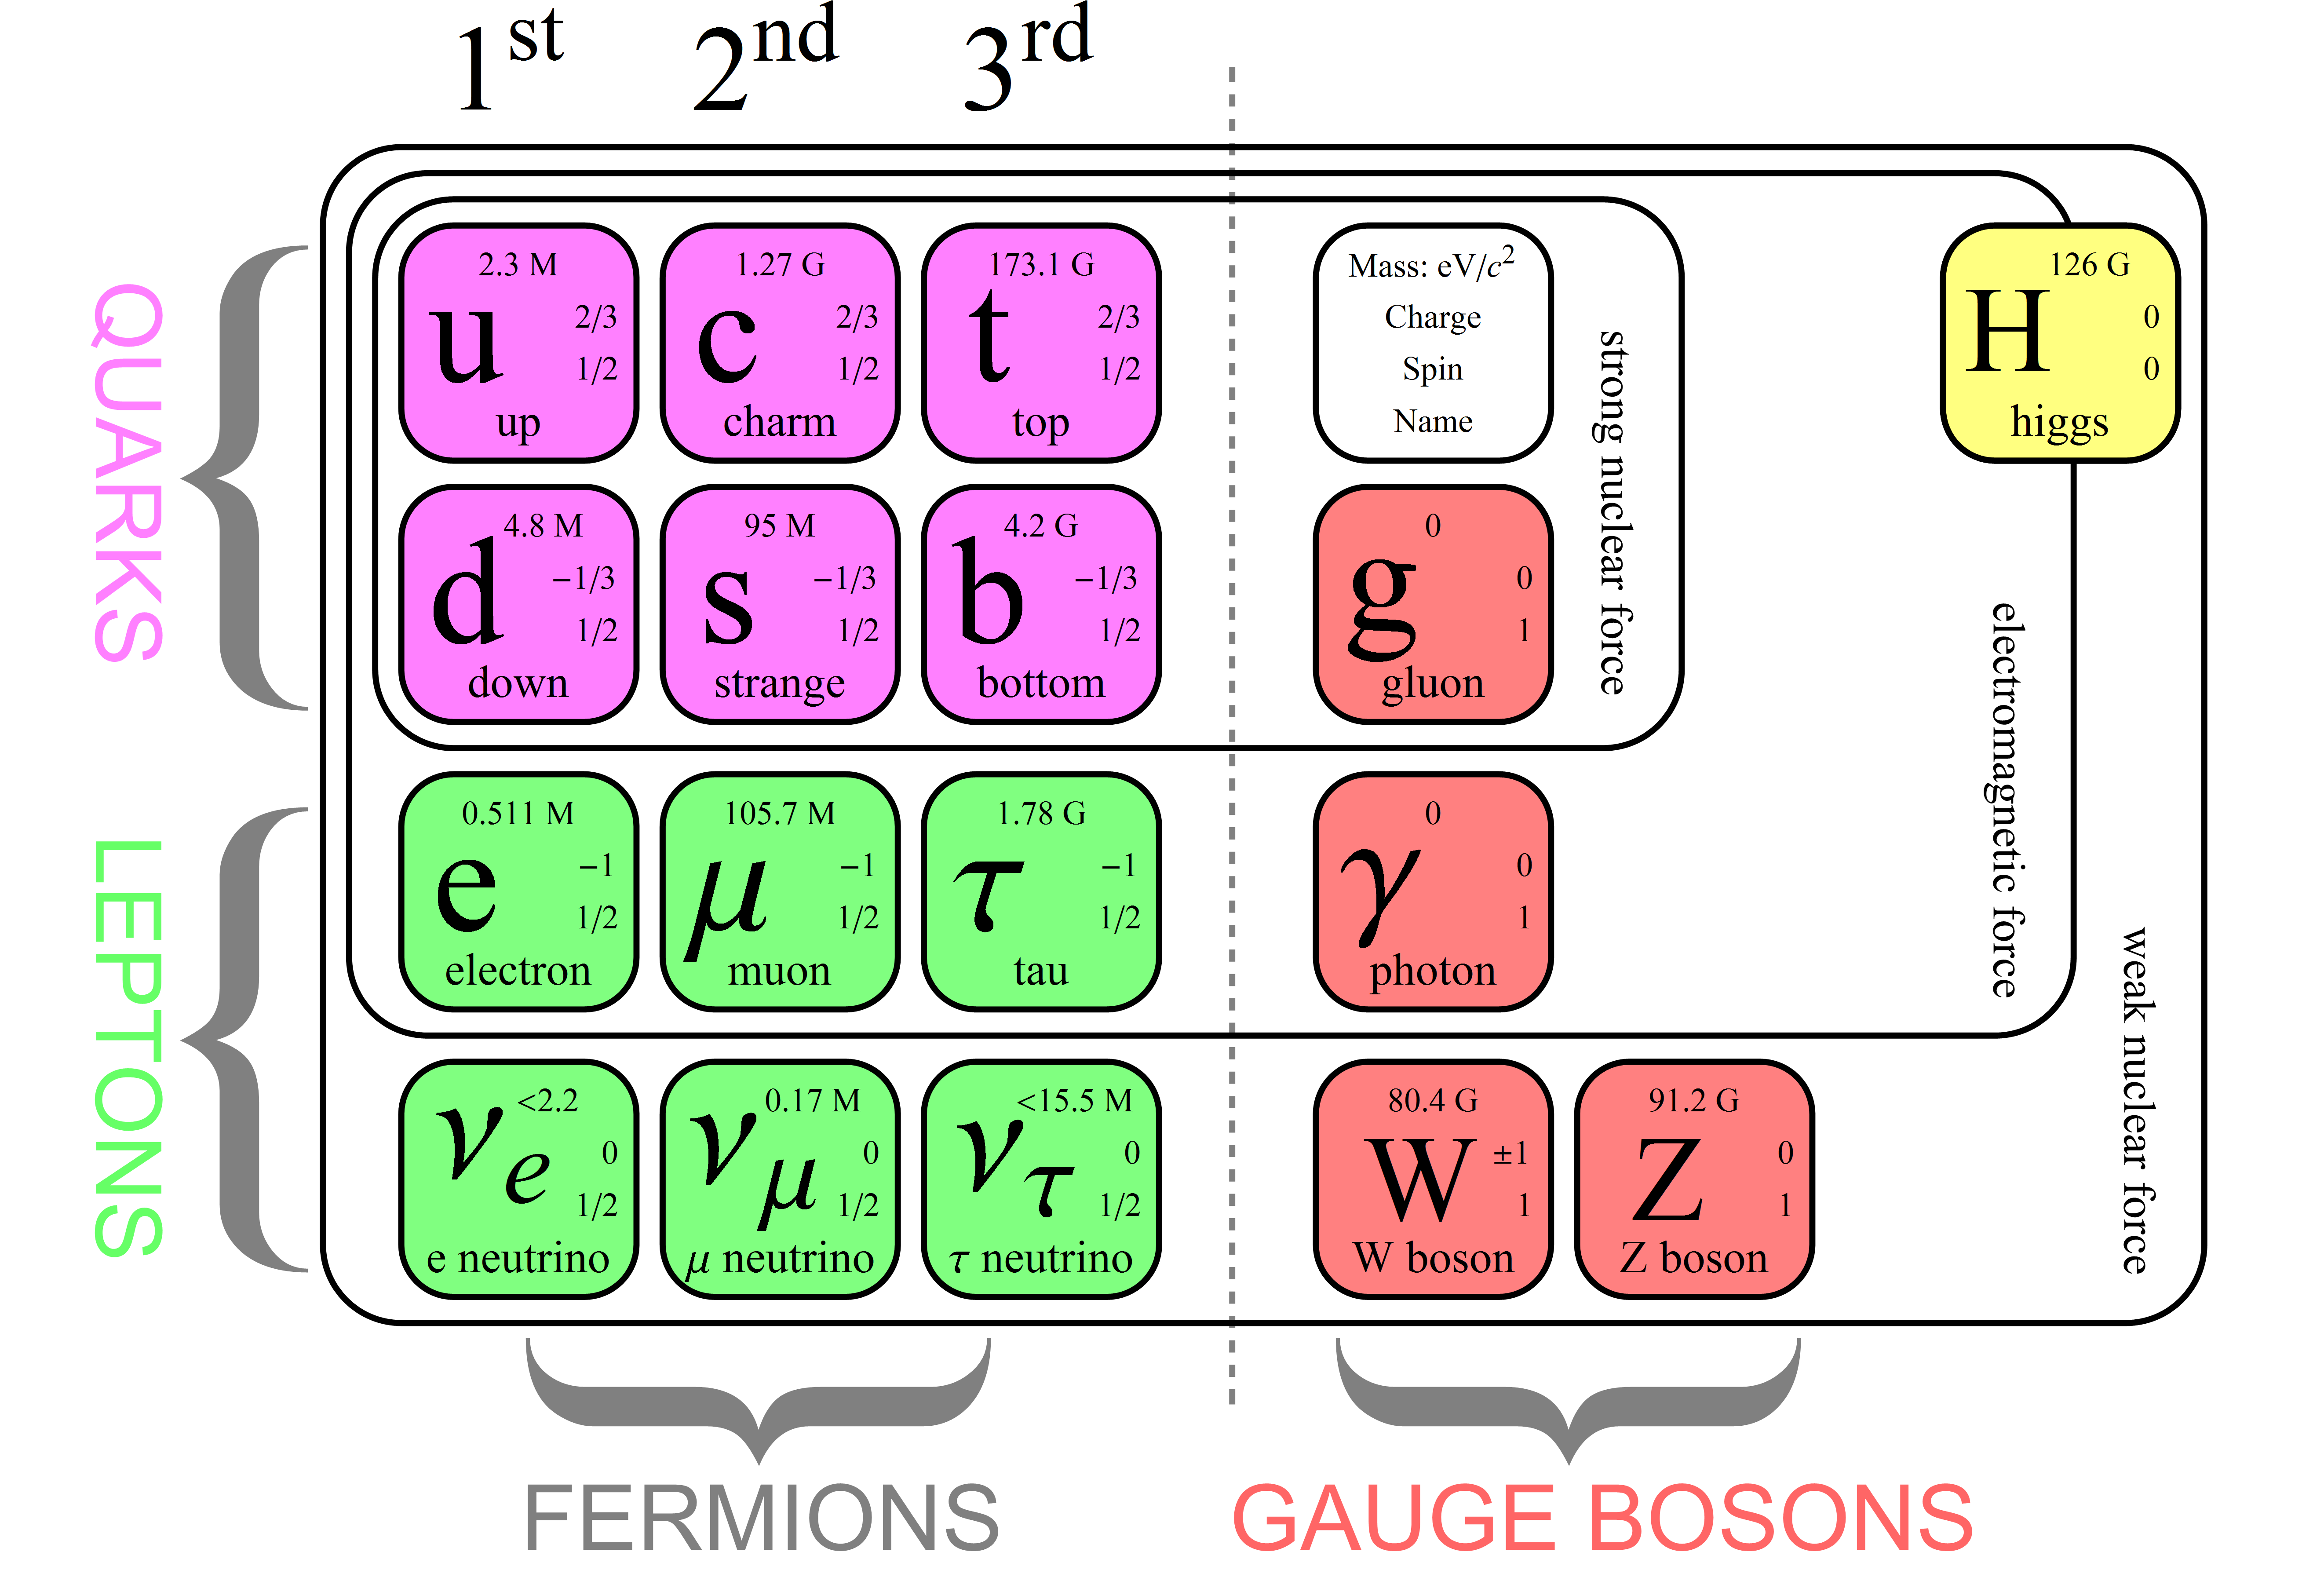
\includegraphics[width=0.9\textwidth]{01StandardModel/figs/particles.png}
  \end{center}
  \vspace{-2mm}
  \caption{Elementary particles described by the SM~\cite{sm-cartoon}.}
  \label{fig:particles}
\end{figure}


All particles are either \emph{fermions} or \emph{bosons}. The fermions (leptons, quarks) have half-integer spin and follow the Fermi-Dirac statistics \cite{Fermi, Dirac}, whereas bosons (gauge bosons, Higgs boson) 
have integer spin and follow the Bose-Einstein statistics \cite{Bose}.

Leptons (spin-$\frac{1}{2}$) include three charged, massive particles (electron $e^-$, muon $\mu^-$ and tau $\tau^-$), which interact via the electromagnetic and weak interactions, and three neutral, (nearly) massless particles, called \emph{neutrinos} ($\nu_{e}$, $\nu_{\mu}$ and $\nu_{\tau}$), which only experience weak interactions.

Six different flavours of quarks (spin-$\frac{1}{2}$) exist: the \emph{up-type} quarks up ($u$), charm ($c$) and  top/truth ($t$), having charge\footnote{Electric charge is always quoted in units of the fundamental charge, defined as minus the charge of the electron.} $+\frac{2}{3}$, and the \emph{down-type} quarks down ($d$), strange ($s$), and bottom/beauty ($b$), which have charge $-\frac{1}{3}$. They can interact via electromagnetic, weak and strong interactions, and they are all massive.

The fundamental interactions are \emph{mediated} by gauge bosons (spin-$1$). The photon ($\gamma$) is responsible for the electromagnetic interaction, whereas the $Z^0$ and $W^\pm$ bosons are the mediators for the weak interaction. These two forces are considered to be different manifestations of a single \emph{electroweak} interaction, which is responsible for all electric and magnetic phenomena as well as some radioactive decays. The strong interaction among quarks is mediated by the gluons $g$. Photon and gluons are massless, whereas the weak force gauge bosons have a non-zero mass.

Each particle has an \emph{antiparticle} partner, which has the same mass as the corresponding particle, but opposite quantum numbers (electric charge, lepton numbers, etc\dots).

Quarks do not exist in a free state: they can only be bound inside \emph{hadrons} via the \emph{confinement} mechanism, a feature of the strong interaction. A hadron can be composed by a quark-antiquark pair (\emph{meson}), or by three quarks or antiquarks (\emph{baryons}). Examples of mesons include the $B^0$ ($\bar b d$) and $D^+$ ($c\bar d$) mesons, whereas the proton ($uud$) and the neutron ($udd$) are examples of baryons. Recently more complex states (tetraquarks~\cite{LHCb-PAPER-2014-014}, pentaquarks~\cite{LHCb-PAPER-2015-029}) have been evidenced.

The non-zero mass of leptons, quarks and weak force gauge bosons would require a gauge symmetry breaking term in the SM Lagrangian density. 
The \emph{Brout-Englert-Higgs mechanism} \cite{BroutEnglert, Higgs, Guralnik} introduces a scalar (spin-$0$) field, called Higgs field, and a potential that allows the Higgs field to have a non-zero vacuum expectation value.
This implies that the gauge symmetry is broken \emph{dynamically}, and that the masses of the particles arise from the resulting interaction with the Higgs field. The quantum of the Higgs field is known as Higgs boson, the last SM particle discovered experimentally \cite{ATLAS, CMS}.

The fourth fundamental interaction, the gravitational force, is described by another field theory, the General Relativity (GR), currently not unified with the SM.

Any experimental signature that is not described by the SM would be a hint for \emph{new physics} (NP). Although the SM is known to be an incomplete theory because of different unsolved problems, such as dark matter, \emph{naturalness}, matter-antimatter asymmetry, lack of SM-GR unification, etc\dots, no evidence for NP has been found so far.
